%% system-matrix.tex — Per-system classification matrix
%% Included from 06-comparison.tex

\subsection{Per-System Classification}
\label{sec:system-matrix}

Table~\ref{tab:system-matrix} presents per-feature classifications for
41~systems with complete capability data across the eight discriminating
features defined in \S\ref{sec:long-tail}.  Systems are grouped by category
and sorted alphabetically within each group.

\begin{table*}[!t]
\centering
\caption{Per-system capability matrix for 41 classified systems.
$\bullet$~=~capability present.
RAG tier: N~=~Naive, A~=~Advanced, M~=~Modular~\cite{gao2023rag}.
An interactive visualization with filtering is available at
\url{https://securityronin.github.io/alaya/docs/memory-landscape.html}.}
\label{tab:system-matrix}
\scriptsize
\setlength{\tabcolsep}{3.5pt}
\begin{tabular}{@{}lc cccccccc@{}}
\toprule
\textbf{System}
  & \rotatebox{90}{\textbf{RAG}}
  & \rotatebox{90}{\textbf{Episodic}}
  & \rotatebox{90}{\textbf{Semantic}}
  & \rotatebox{90}{\textbf{Graph}}
  & \rotatebox{90}{\textbf{Fusion}}
  & \rotatebox{90}{\textbf{Consolid.}}
  & \rotatebox{90}{\textbf{Forgetting}}
  & \rotatebox{90}{\textbf{Contrad.}}
  & \rotatebox{90}{\textbf{Preference}} \\
\midrule
\multicolumn{10}{@{}l}{\textit{Dedicated Memory Systems (25)}} \\
ChatGPT Memory       & N & $\bullet$ &           &           &           &           & $\bullet$ &           & $\bullet$ \\
Claude Memory Tool   & N & $\bullet$ &           &           &           &           &           &           &           \\
Cognee               & A &           & $\bullet$ & $\bullet$ & $\bullet$ &           &           &           &           \\
Cortex-Mem           & N &           & $\bullet$ &           &           &           &           &           &           \\
EverMemOS            & A & $\bullet$ & $\bullet$ &           & $\bullet$ & $\bullet$ & $\bullet$ &           &           \\
Gemini Memory        & N & $\bullet$ &           &           &           &           &           &           & $\bullet$ \\
Grok Memory          & N & $\bullet$ &           &           &           &           &           &           & $\bullet$ \\
Hindsight            & A & $\bullet$ & $\bullet$ &           & $\bullet$ &           & $\bullet$ & $\bullet$ & $\bullet$ \\
MCP Mem.\ Service    & A &           & $\bullet$ & $\bullet$ & $\bullet$ &           &           &           &           \\
Mem0                 & A & $\bullet$ & $\bullet$ & $\bullet$ & $\bullet$ &           & $\bullet$ & $\bullet$ & $\bullet$ \\
Memary               & A &           & $\bullet$ & $\bullet$ &           &           & $\bullet$ &           &           \\
Memobase             & N &           &           &           &           &           &           &           & $\bullet$ \\
MemOS                & A & $\bullet$ & $\bullet$ & $\bullet$ & $\bullet$ & $\bullet$ & $\bullet$ &           & $\bullet$ \\
MemoryOS             & A & $\bullet$ & $\bullet$ &           & $\bullet$ &           & $\bullet$ &           & $\bullet$ \\
Memonto              & N &           & $\bullet$ & $\bullet$ &           &           &           &           &           \\
Memvid               & A & $\bullet$ &           &           & $\bullet$ &           &           &           &           \\
Meta AI Memory       & N & $\bullet$ &           &           &           &           &           &           &           \\
Neo4j Agent Mem.     & A & $\bullet$ & $\bullet$ & $\bullet$ & $\bullet$ &           &           &           &           \\
OpenClaw Redis       & A & $\bullet$ & $\bullet$ &           &           &           & $\bullet$ &           & $\bullet$ \\
OpenMemory           & A & $\bullet$ & $\bullet$ & $\bullet$ & $\bullet$ &           & $\bullet$ &           & $\bullet$ \\
Perplexity Memory    & A & $\bullet$ &           &           &           &           &           &           & $\bullet$ \\
Redis Memory         & A &           & $\bullet$ &           & $\bullet$ &           &           &           &           \\
Supermemory          & A & $\bullet$ & $\bullet$ & $\bullet$ &           &           & $\bullet$ &           & $\bullet$ \\
Vestige              & M & $\bullet$ & $\bullet$ & $\bullet$ & $\bullet$ &           & $\bullet$ &           & $\bullet$ \\
Zep/Graphiti         & M & $\bullet$ & $\bullet$ & $\bullet$ & $\bullet$ & $\bullet$ & $\bullet$ & $\bullet$ &           \\
\midrule
\multicolumn{10}{@{}l}{\textit{Framework Memory Modules (6)}} \\
CrewAI               & A & $\bullet$ & $\bullet$ &           & $\bullet$ &           &           &           & $\bullet$ \\
LangChain            & N & $\bullet$ &           &           &           &           & $\bullet$ &           &           \\
LangMem SDK          & N &           & $\bullet$ &           &           &           &           &           &           \\
Letta (MemGPT)       & N & $\bullet$ & $\bullet$ &           &           & $\bullet$ & $\bullet$ &           & $\bullet$ \\
LlamaIndex           & N & $\bullet$ &           &           &           &           & $\bullet$ &           &           \\
MS GraphRAG          & M &           & $\bullet$ & $\bullet$ & $\bullet$ &           &           &           &           \\
\midrule
\multicolumn{10}{@{}l}{\textit{Coding Agent Memory (4)}} \\
Beads                & A & $\bullet$ & $\bullet$ & $\bullet$ &           & $\bullet$ & $\bullet$ &           &           \\
Cipher (ByteRover)   & A & $\bullet$ & $\bullet$ &           &           &           & $\bullet$ &           &           \\
Engram               & N & $\bullet$ &           &           &           &           &           &           &           \\
Memsearch            & A & $\bullet$ &           &           &           &           & $\bullet$ &           &           \\
\midrule
\multicolumn{10}{@{}l}{\textit{File-Based Memory (2)}} \\
Claude Code          & N & $\bullet$ &           &           &           &           &           &           & $\bullet$ \\
Claudesidian         & A & $\bullet$ &           & $\bullet$ &           &           & $\bullet$ &           &           \\
\midrule
\multicolumn{10}{@{}l}{\textit{Research Architectures (10)}} \\
A-MEM                & A &           & $\bullet$ & $\bullet$ & $\bullet$ &           &           &           &           \\
Generative Agents    & A & $\bullet$ & $\bullet$ &           & $\bullet$ & $\bullet$ & $\bullet$ &           & $\bullet$ \\
HippoRAG             & M &           & $\bullet$ & $\bullet$ &           &           &           &           &           \\
HippoRAG~2           & M & $\bullet$ & $\bullet$ & $\bullet$ & $\bullet$ &           &           &           &           \\
LightMem             & A & $\bullet$ & $\bullet$ &           &           & $\bullet$ & $\bullet$ &           &           \\
LightRAG             & M &           & $\bullet$ & $\bullet$ & $\bullet$ &           &           &           &           \\
Mem-alpha            & A & $\bullet$ & $\bullet$ &           &           &           & $\bullet$ &           &           \\
MemAgent             & A & $\bullet$ &           &           &           &           & $\bullet$ &           &           \\
MemoRAG              & A & $\bullet$ & $\bullet$ &           & $\bullet$ &           &           &           &           \\
SYNAPSE              & M & $\bullet$ & $\bullet$ & $\bullet$ & $\bullet$ & $\bullet$ & $\bullet$ &           &           \\
\bottomrule
\end{tabular}
\end{table*}

Three patterns emerge from the per-system view that are not visible in the
aggregate statistics.  First, contradiction resolution is the rarest
capability: only 3 of 41~systems implement it (Mem0, Zep/Graphiti,
and Hindsight), all dedicated memory systems.  Second, Modular RAG systems
implement more lifecycle operations (consolidation, forgetting) than Naive
or Advanced RAG systems---retrieval sophistication correlates with
architectural investment in lifecycle operations.  Third, framework memory
modules implement at most five of the eight features: memory is a secondary
concern in orchestration frameworks, limiting investment in consolidation,
contradiction resolution, and graph-based retrieval.

\begin{figure}[!t]
\centering
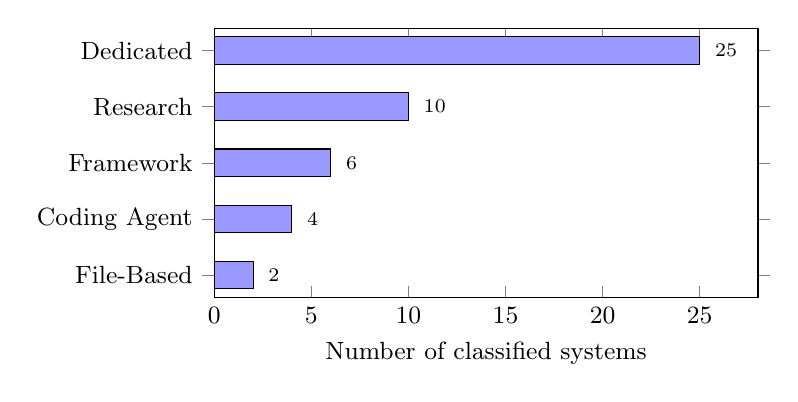
\begin{tikzpicture}
\begin{axis}[
    xbar,
    width=0.7\columnwidth,
    height=5cm,
    xlabel={Number of classified systems},
    symbolic y coords={File-Based, Coding Agent, Framework, Research, Dedicated},
    ytick=data,
    xmin=0, xmax=28,
    nodes near coords,
    nodes near coords style={font=\scriptsize, anchor=west},
    every node near coord/.append style={xshift=2pt},
    bar width=10pt,
    x tick label style={font=\small},
    y tick label style={font=\small},
    xlabel style={font=\small},
]
\addplot[fill=blue!40] coordinates {
    (2,File-Based)
    (4,Coding Agent)
    (6,Framework)
    (10,Research)
    (25,Dedicated)
};
\end{axis}
\end{tikzpicture}
\caption{Number of classified systems by category.  Dedicated memory systems
dominate the landscape, reflecting the field's focus on memory as a primary
architectural concern.  Framework modules and coding agent tools are
underrepresented, consistent with memory being an auxiliary feature in
these categories.}
\label{fig:category-scores}
\end{figure}

Figure~\ref{fig:category-scores} summarizes the category-level pattern:
dedicated systems dominate the classified landscape, while framework modules
and coding tools remain underrepresented---consistent with memory being a
secondary concern in orchestration and development tool contexts.  For
interactive exploration with filtering by category, capability, and RAG tier,
see the companion
visualization.\footnote{\url{https://securityronin.github.io/alaya/docs/memory-landscape.html}}
